% !TeX document-id = {9bb2973f-2b37-4107-8210-f9ba2cdb8d34}
% !TeX TXS-program:compile = txs:///pdflatex/[--shell-escape]
%% !TEX TS-program = xelatex
% !TEX encoding = UTF-8 Unicode

% Spring 2020 - Summer 2020 - Fall 2020
% Tristan Hill, May 07, 2020 - June 12, 2020 - July 08, 2020 - Novemeber 02, 2020
% Module 11 - Probability and Statistics
% Topic 2 - Characterizing a Population of Data

\documentclass[fleqn]{beamer} % for presentation (has nav buttons at bottom)
\usepackage{../../measurements_lectures}

\author{ME3023 - Measurements in Mechanical Systems} % original formatting from Mike Renfro, September 21, 2004

\newcommand{\MNUM}{11\hspace{2mm}} % Module number
\newcommand{\TNUM}{2\hspace{2mm}} % Topic number 
\newcommand{\moduletitle}{Probability and Statistics}
\newcommand{\topictitle}{Characterizing a Population of Data} 

\newcommand{\sectiontitleI}{A Population of Data}
\newcommand{\sectiontitleII}{Variance and Standard Deviation}
\newcommand{\sectiontitleIII}{Using the Z Table}
\newcommand{\sectiontitleIV}{Example: Using the Z Table}

% custom box
\newsavebox{\mybox}

\title{Lecture Module - \moduletitle}

\date{Mechanical Engineering\vspc Tennessee Technological University}

\begin{document}
	
	\lstset{language=MATLAB,basicstyle=\ttfamily\small,showstringspaces=false}
	
	\frame{\titlepage \center\begin{framed}\Large \textbf{Topic \TNUM - \topictitle}\end{framed} \vspace{5mm}}

% Section 0: Outline
\frame{
\large \textbf{Topic \TNUM - \topictitle} \vspace{3mm}\\

\begin{itemize}

	\item \sectiontitleI    \vspc % Section I
	\item \sectiontitleII 	\vspc % Section II
	\item \sectiontitleIII 	\vspc %Section III
	\item \sectiontitleIV 	\vspc %Section IV

\end{itemize}

}

\section{\sectiontitleI}	
	% Section I - Frame I
	\begin{frame}[label=sectionI] \small
		\frametitle{\sectiontitleI}    
		
		Consider a manufacturing facility that makes ball bearings. 
		\begin{itemize}		
			\item How does the manufacturer ensure the quality of the product?
			\item How the does the seller communicate this to the buyer?
			\item How does the Engineer use this information? 
		\end{itemize}		
		
	\end{frame}
	
	% Section I - Frame II
	\begin{frame}\small
		\frametitle{\sectiontitleI}    
		
		\textbf{For a given set of measurements we want to quantify:}
		\begin{itemize}
			\item a representative value that characterizes the average of the measured data set
			\item a representative value that provides a measure of the variation in the data set
			\item how well the average of the measured data set represents the average of the entire population
		\end{itemize}
		
	\end{frame}


\section{\sectiontitleII}	
	% Section II - Frame I
	\begin{frame}[label=sectionII] \small
		\frametitle{\sectiontitleII}    
		
		\begin{multicols}{2} \tiny
		The true variance is:\\
		\[ \sigma^2=\int\limits_{-\infty}^{\infty}(x-x')^2p(x)dx \]
		For discrete data this becomes:\\
		\[ \sigma^2=\lim\limits_{N\rightarrow \infty}\frac{1}{N}\sum\limits_{i=1}^{N}(x_i-x')^2 \]
		The square root of the {\bf \BL variance} \\
		is the {\bf \PR standard deviation}. \\
		\[\sigma=\sqrt{\sigma^2}\]

		\hspace*{-1.5cm}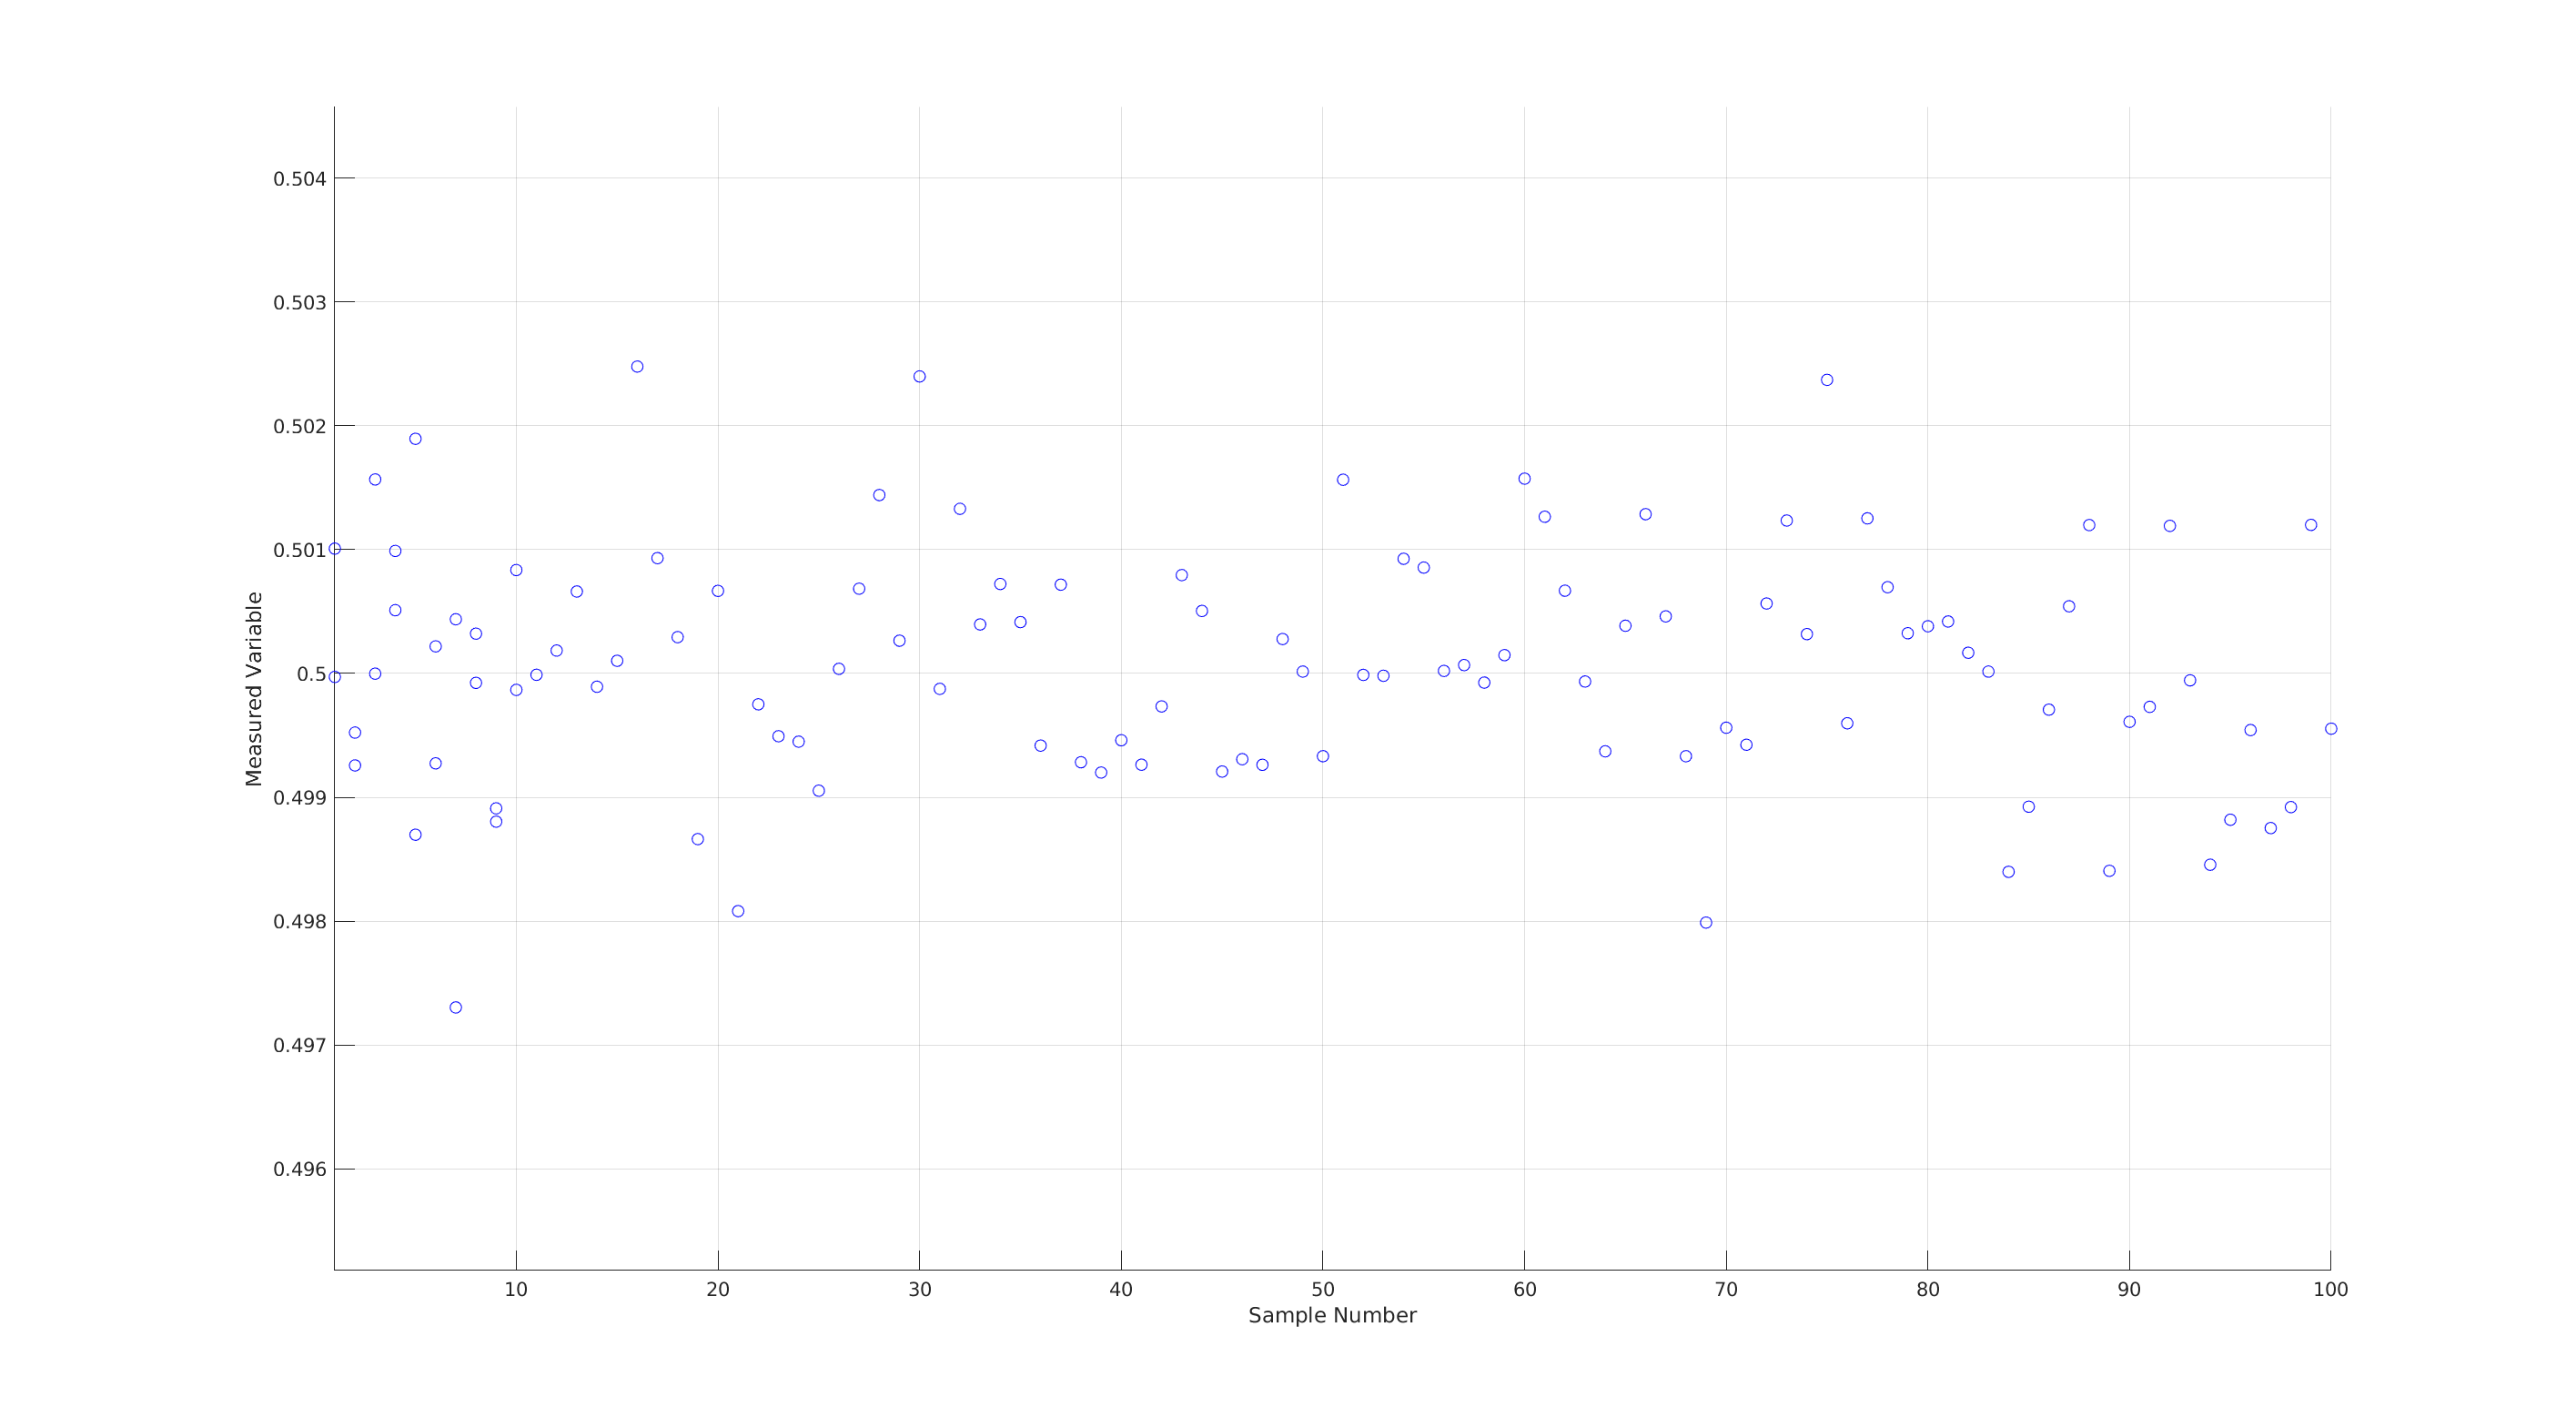
\includegraphics[scale=.20]{topic2_measured_fig2.png}		
		
		\end{multicols}


	\end{frame}
	
	% Section II - Frame II
	\begin{frame} \small
		\frametitle{\sectiontitleII}    

		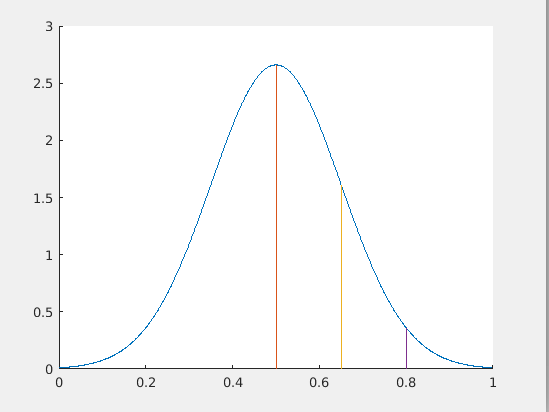
\includegraphics[scale=.50]{lecture1_fig1.png}		
		
	\end{frame}
	
	% Section II - Frame III
	\begin{frame} \small
		\frametitle{\sectiontitleII}    

		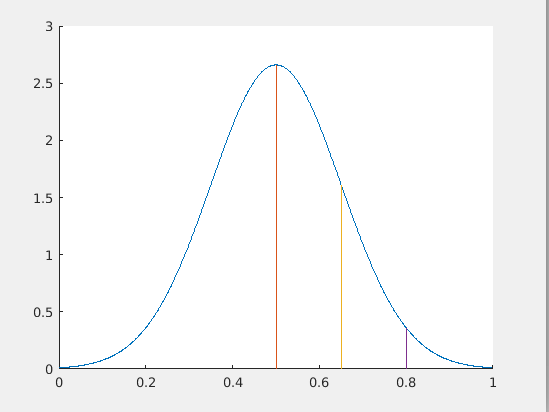
\includegraphics[scale=.50]{lecture1_fig1.png}		
		
	\end{frame}


\section{\sectiontitleIII}	

	% Section III - Frame I
	\begin{frame}[label=sectionIII] \small
		\frametitle{\sectiontitleIII}    
	
		%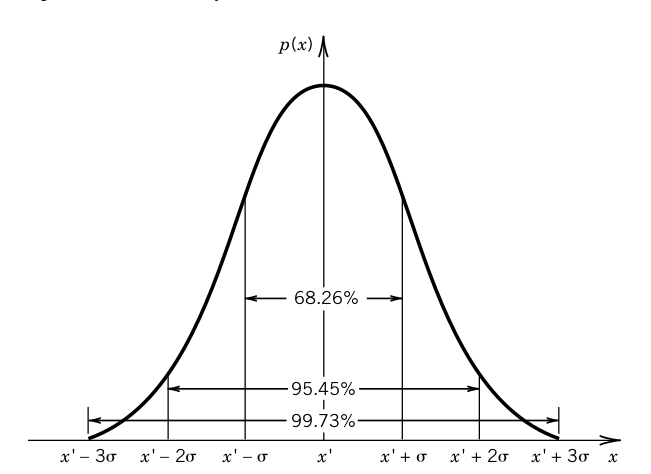
\includegraphics[scale=.250]{topic2_fig4.png}
		
		... The area under the portion of the probability density function curve, $p(x)$, defined by the interval $x'-z_1\sigma \leq x \leq x' +z_1\sigma$ provides the probability that a measurement will assume a value within that interval. Direct integration of $p(x)$ for a normal
distribution between the limits $x'\pm z_1\sigma$ yields that for $z_1=1, 68.26\%$ of the area under $p(x)$ lies
within $\pm 1\sigma$   $x'$ . This means that there is a $68.26\%$ chance that a measurement of $x$ will have a
value within the interval $x'\pm 1\sigma$.
			

	\end{frame}


	% Section III - Frame II
	\begin{frame}[label=sectionIII] \small
		\frametitle{\sectiontitleIII}    
	
		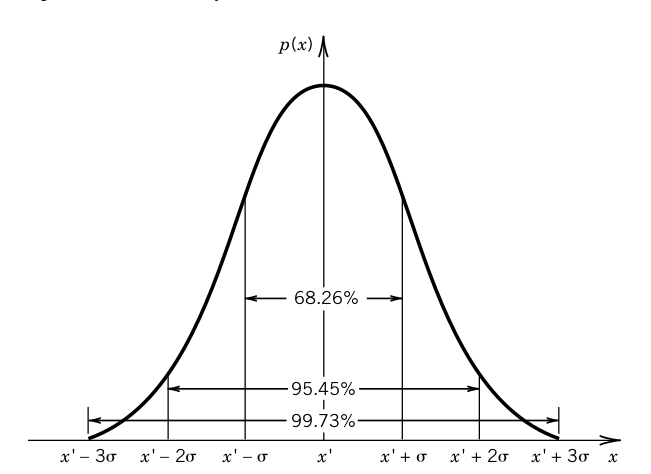
\includegraphics[scale=.250]{topic2_fig4.png}
		
		$ z_1=1, 68.26\% $ of the area under $ p(x) $ lies within $ \pm z_1\sigma $ of $ x' $.\\ 
		$ z_1=2, 95.45\% $ of the area under $ p(x) $ lies within $ \pm z_1\sigma $ of $ x' $.\\ 
		$ z_1=3, 99.73\% $ of the area under $ p(x) $ lies within $ \pm z_1\sigma $ of $ x' $.\\ 		
		

	\end{frame}
	
	% Section III - Frame III
	\begin{frame}[label=sectionIII] \small
		\frametitle{\sectiontitleIII}    
	
		It follows directly that the representative value that characterizes a measure of the variation in a
measured data set is the standard deviation. The probability that the ith measured value of x will
have a value between $x' \pm z_1 \delta$ is $2 \times P(z_1) \times 100 = P\%$. \\

	This is written as \\
	
		\[ x_i = x' \pm z_1\sigma \hspace{3mm} (P\%) \]        
		
			

	\end{frame}


\section{\sectiontitleIV}	
	% Section IV - Frame I
	\begin{frame}[label=sectionIV] \small
		\frametitle{\sectiontitleIV}    

		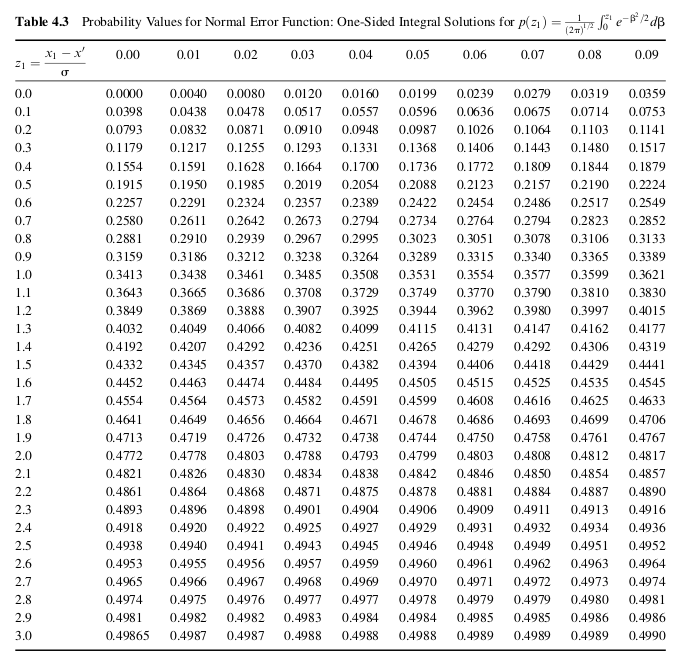
\includegraphics[scale=.25]{topic2_fig2.png}	
		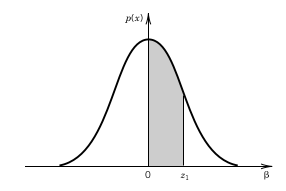
\includegraphics[scale=.45]{topic2_fig3.png}	

	\end{frame}


\end{document}




	





